% WACV 2027 Paper Template
% based on the ICCV 2025 template (https://media.eventhosts.cc/Conferences/ICCV2025/ICCV2025-Author-Kit-Feb.zip) with
% WACV-specific details (e.g., 2 tracks) from the WACV 2025 template (https://www.dropbox.com/scl/fi/su44zgdhrzik26p2xu37k/WACV-2025-Author-Kit-Template.zip?rlkey=5qcfimjhxnmx3wlyk7yhk8wg7&dl=0)

\documentclass[10pt,twocolumn,letterpaper]{article}

%%%%%%%%% PAPER TYPE  - PLEASE UPDATE FOR FINAL VERSION
% \usepackage[review,algorithms]{wacv}      % To produce the REVIEW version for the algorithms track
% \usepackage[review,applications]{wacv}      % To produce the REVIEW version for the applications track
% \usepackage[review,datasets]{wacv}      % To produce the REVIEW version for the datasets track
\usepackage{wacv}              % To produce the CAMERA-READY version
% \usepackage[pagenumbers]{wacv}

% Import additional packages in the preamble file, before hyperref
%
% --- inline annotations
%
\newcommand{\red}[1]{{\color{red}#1}}
\newcommand{\todo}[1]{{\color{red}#1}}
\newcommand{\TODO}[1]{\textbf{\color{red}[TODO: #1]}}
% --- disable by uncommenting  
% \renewcommand{\TODO}[1]{}
% \renewcommand{\todo}[1]{#1}



\usepackage{multirow}


% It is strongly recommended to use hyperref, especially for the review version.
% hyperref with option pagebackref eases the reviewers' job.
% Please disable hyperref *only* if you encounter grave issues,
% e.g. with the file validation for the camera-ready version.
%
% If you comment hyperref and then uncomment it, you should delete *.aux before re-running LaTeX.
% (Or just hit 'q' on the first LaTeX run, let it finish, and you should be clear).
\definecolor{wacvblue}{rgb}{0.21,0.49,0.74}
\usepackage[pagebackref,breaklinks,colorlinks,allcolors=wacvblue]{hyperref}

%%%%%%%%% PAPER ID  - PLEASE UPDATE
\def\wacvPaperID{*****} % *** Enter the WACV Paper ID here
\def\confName{WACV}
\def\confYear{2027}


%%%%%%%%% TITLE - PLEASE UPDATE
\title{CortexDecoder: fMRI-to-image Reconstruction from Cortical Flatmaps}

%%%%%%%%% AUTHORS - PLEASE UPDATE
\author{Teo Imoto-Tar\\
UC San Diego\\
{\tt\small timototar@ucsd.edu}
\and
Maxwell Fung\\
UC Berkeley\\
{\tt\small maxwellfung@berkeley.edu} \\
\and
Arnav Gurha \\
UC San Diego \\
{\tt\small agurha@ucsd.edu}
}

\begin{document}
\maketitle
\begin{abstract}
Recent advances in brain decoding have shown the potential of vision transformers (ViTs) to learn mappings from neural representations to visual features. Here we present CortexDecoder, a brain decoding framework that maps fMRI flatmaps to the images viewed by subjects. Flatmaps are neural responses projected onto the cortical surface and then unfolded into 2D images. We demonstrate that (1) flatmaps preserve sufficient signal to achieve high performance in brain decoding, whereas raw fMRI data is noisy and high-dimensional, which makes decoding difficult; and (2) reshaping raw fMRI data into flatmaps allows for clean patch-based tokenization. This lets us harness state-of-the-art ViTs to learn meaningful neural representations while preserving spatial encoding. To do this, we pass flatmap patches into a pretrained CortexMAE encoder to obtain brain tokens. A lightweight cross-attention bridge then learns to map these brain tokens to image features. The bridge is split into two modules: a semantic module that predicts CLIP embeddings and a low-level module that generates a low-level image reconstruction. Finally, a fine-tuned SDXL (Stable Diffusion XL) model takes this low-level reconstruction as its initial image and, conditioned on the predicted CLIP embedding, produces the final reconstruction. In evaluations on two NSD subjects, CortexDecoder achieves performance comparable to state-of-the-art brain decoding methods, demonstrating the efficacy of flatmap-based neural representations for visual reconstruction.
\end{abstract}

\section{Introduction}
\label{sec:intro}

\begin{center}
\begin{figure*}[t]
    \centering
    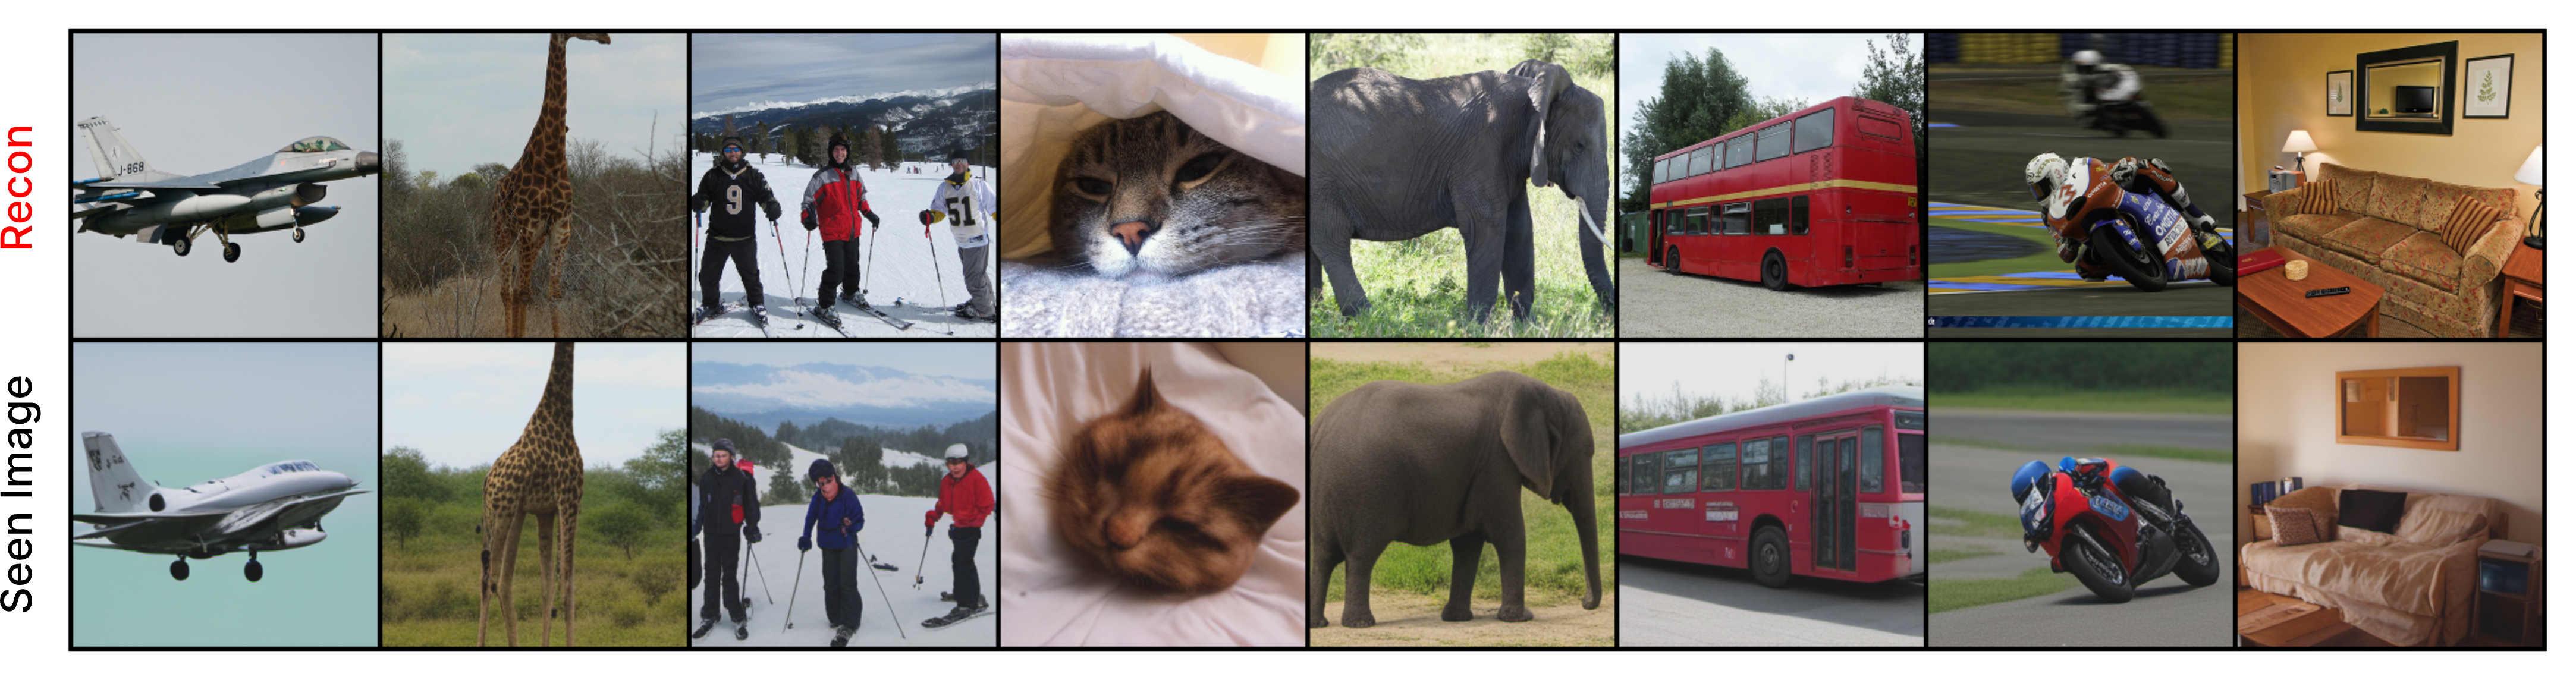
\includegraphics[width=0.9\textwidth]{images/title4.png}
    \caption{Stimuli (top) and CortexDecoder reconstructions (bottom). Images from COCO \cite{lin2015microsoftcococommonobjects} (CC BY 4.0).}
    \label{fig:title}
\end{figure*}
\end{center}

Reconstructing visual experiences from non-invasive functional Magnetic Resonance Imaging (fMRI) remains a central challenge in computational neuroscience. It is also vital for Brain-Computer Interfaces (BCIs), such as communication aids. With the availability of large, open-source fMRI-image datasets like the Natural Scenes Dataset (NSD) \cite{Allen2022Massive7TfMRI}, fMRI has become a natural choice for studying visual decoding. The NSD provides paired fMRI responses and natural images viewed by subjects, with repeated presentations of visual stimuli across trials. Each sample contains a cortical response corresponding to a viewed image, providing both neural and visual representations for learning fMRI-to-image mappings.

Our central question is: how much information about visual stimuli can we decode from 2D cortical flatmaps? Most brain decoding frameworks follow one of two practices. Some approaches regress directly from raw 3D functional volumes, but this is challenging due to their high dimensionality, noisy voxel-wise signal, and computational cost. Alternatively, conventional approaches that flatten voxel responses into feature vectors or average responses over anatomical parcellations do not explicitly preserve spatial information. This motivated us to explore 2D flatmaps, which preserve cortical geometry and are directly compatible with modern vision architectures.

We introduce CortexDecoder, a framework that decodes 2D cortical flatmaps into image stimuli using vision transformer (ViT) \cite{dosovitskiy2021imageworth16x16words} models. Since flatmaps are inherently 2D images, we can partition neural activity into discrete patches. We use a pretrained CortexMAE \cite{lane2026scalingvisiontransformersfunctional} encoder---an fMRI foundation model developed by MedARC using the masked autoencoder framework specifically for cortical flatmaps. From this encoder, we extract spatially organized brain tokens. By retaining the full sequence of spatially organized patch tokens from CortexMAE, our architecture preserves local cortical geometry. This avoids collapsing the brain representation into a rigid 1D feature vector, which discards its underlying spatial organization.

Our cross-attention bridge, heavily inspired by DETR (DEtection TRansformer) \cite{DBLP:journals/corr/abs-2005-12872} and Brain-IT \cite{beliy2025brainitimagereconstructionfmri}, uses learned query vectors to map neural representations to visual feature spaces. Our cross-attention bridge is split into two modules to separately handle semantic and structural visual information. The semantic branch predicts unpooled CLIP \cite{radford2021learningtransferablevisualmodels} embeddings to capture the scene’s meaning, whereas the low-level branch targets early visual features such as basic shapes and colors. Many decoding models struggle with low-level visual fidelity, often generating images that match semantically but are unfaithful in terms of pixel correlation and structural similarity. Incorporating a low-level branch targets this gap by providing structural guidance. Finally, we employ MindEye2’s \cite{scotti2024mindeye2sharedsubjectmodelsenable} fine-tuned SDXL \cite{podell2023sdxlimprovinglatentdiffusion} to condition on both the low-level reconstruction and a semantic embedding to produce the final image.

Our main contributions are as follows: (1) we propose CortexDecoder, a novel architecture that uses 2D cortical flatmaps as input for fMRI-to-image reconstruction; (2) we show that flatmaps preserve enough signal for reconstruction, achieving competitive benchmark results; and (3) we show that flatmaps allow for clean tokenization and are compatible with Vision Transformers out of the box.



% %-------------------------------------------------------------------------
% \subsection{Language}

% All manuscripts must be in English.

% \subsection{Dual submission}

% Please refer to the author guidelines on the \confName\ \confYear\ web page for a
% discussion of the policy on dual submissions.

% \subsection{Paper length}
% Papers, excluding the references section, must be no longer than eight pages in length.
% The references section will not be included in the page count, and there is no limit on the length of the references section.
% For example, a paper of eight pages with two pages of references would have a total length of 10 pages.
% {\bf There will be no extra page charges for \confName\ \confYear.}

% Overlength papers will simply not be reviewed.
% This includes papers where the margins and formatting are deemed to have been significantly altered from those laid down by this style guide.
% Note that this \LaTeX\ guide already sets figure captions and references in a smaller font.
% The reason such papers will not be reviewed is that there is no provision for supervised revisions of manuscripts.
% The reviewing process cannot determine the suitability of the paper for presentation in eight pages if it is reviewed in eleven.

% %-------------------------------------------------------------------------
% \subsection{The ruler}
% The \LaTeX\ style defines a printed ruler which should be present in the version submitted for review.
% The ruler is provided in order that reviewers may comment on particular lines in the paper without circumlocution.
% If you are preparing a document using a non-\LaTeX\ document preparation system, please arrange for an equivalent ruler to appear on the final output pages.
% The presence or absence of the ruler should not change the appearance of any other content on the page.
% The camera-ready copy should not contain a ruler.
% (\LaTeX\ users may use options of \texttt{wacv.sty} to switch between different versions.)

% Reviewers:
% note that the ruler measurements do not align well with lines in the paper --- this turns out to be very difficult to do well when the paper contains many figures and equations, and, when done, looks ugly.
% Just use fractional references (\eg, this line is $087.5$), although in most cases one would expect that the approximate location will be adequate.


% \subsection{Paper ID}
% Make sure that the Paper ID from the submission system is visible in the version submitted for review (replacing the ``*****'' you see in this document).
% If you are using the \LaTeX\ template, \textbf{make sure to update paper ID in the appropriate place in the tex file}.


% \subsection{Mathematics}

% Please number all of your sections and displayed equations as in these examples:
% \begin{equation}
%   E = m\cdot c^2
%   \label{eq:important}
% \end{equation}
% and
% \begin{equation}
%   v = a\cdot t.
%   \label{eq:also-important}
% \end{equation}
% It is important for readers to be able to refer to any particular equation.
% Just because you did not refer to it in the text does not mean some future reader might not need to refer to it.
% It is cumbersome to have to use circumlocutions like ``the equation second from the top of page 3 column 1''.
% (Note that the ruler will not be present in the final copy, so is not an alternative to equation numbers).
% All authors will benefit from reading Mermin's description of how to write mathematics:
% \url{http://www.pamitc.org/documents/mermin.pdf}.

% \subsection{Blind review}

% Many authors misunderstand the concept of anonymizing for blind review.
% Blind review does not mean that one must remove citations to one's own work---in fact it is often impossible to review a paper unless the previous citations are known and available.

% Blind review means that you do not use the words ``my'' or ``our'' when citing previous work.
% That is all.
% (But see below for tech reports.)

% Saying ``this builds on the work of Lucy Smith [1]'' does not say that you are Lucy Smith;
% it says that you are building on her work.
% If you are Smith and Jones, do not say ``as we show in [7]'', say ``as Smith and Jones show in [7]'' and at the end of the paper, include reference 7 as you would any other cited work.


% An example of an acceptable paper:
% \begin{quote}
% \begin{center}
%      An analysis of the frobnicatable foo filter.
% \end{center}

%    In this paper we present a performance analysis of the  paper of Smith \etal [1], and show it to be inferior to all previously known methods.
%    Why the previous paper was accepted without this analysis is beyond me.

%    [1] Smith, L and Jones, C. ``The frobnicatable foo filter, a fundamental contribution to human knowledge''. Nature 381(12), 1-213.
% \end{quote}

% If you are making a submission to another conference at the same time, which covers similar or overlapping material, you may need to refer to that submission in order to explain the differences, just as you would if you had previously published related work.
% In such cases, include the anonymized parallel submission~\cite{Authors14} as supplemental material and cite it as
% \begin{quote}
% [1] Authors. ``The frobnicatable foo filter'', F\&G 2014 Submission ID 324, Supplied as supplemental material {\tt fg324.pdf}.
% \end{quote}

% Finally, you may feel you need to tell the reader that more details can be found elsewhere, and refer them to a technical report.
% For conference submissions, the paper must stand on its own, and not {\em require} the reviewer to go to a tech report for further details.
% Thus, you may say in the body of the paper ``further details may be found in~\cite{Authors14b}''.
% Then submit the tech report as supplemental material.
% Again, you may not assume the reviewers will read this material.

% Sometimes your paper is about a problem which you tested using a tool that is widely known to be restricted to a single institution.
% For example, let's say it's 1969, you have solved a key problem on the Apollo lander, and you believe that the 1970 audience would like to hear about your
% solution.
% The work is a development of your celebrated 1968 paper entitled ``Zero-g frobnication: How being the only people in the world with access to the Apollo lander source code makes us a wow at parties'', by Zeus \etal.

% You can handle this paper like any other.
% Do not write ``We show how to improve our previous work [Anonymous, 1968].
% This time we tested the algorithm on a lunar lander [name of lander removed for blind review]''.
% That would be silly, and would immediately identify the authors.
% Instead write the following:
% \begin{quotation}
% \noindent
%    We describe a system for zero-g frobnication.
%    This system is new because it handles the following cases:
%    A, B.  Previous systems [Zeus et al. 1968] did not  handle case B properly.
%    Ours handles it by including a foo term in the bar integral.

%    ...

%    The proposed system was integrated with the Apollo lunar lander, and went all the way to the moon, don't you know.
%    It displayed the following behaviours, which show how well we solved cases A and B: ...
% \end{quotation}
% As you can see, the above text follows standard scientific convention, reads better than the first version, and does not explicitly name you as the authors.
% A reviewer might think it likely that the new paper was written by Zeus \etal, but cannot make any decision based on that guess.
% He or she would have to be sure that no other authors could have been contracted to solve problem B.
% \medskip

% \noindent
% FAQ\medskip\\
% {\bf Q:} Are acknowledgements OK?\\
% {\bf A:} No.  Leave them for the final copy.\medskip\\
% {\bf Q:} How do I cite my results reported in open challenges?
% {\bf A:} To conform with the double-blind review policy, you can report results of other challenge participants together with your results in your paper.
% For your results, however, you should not identify yourself and should not mention your participation in the challenge.
% Instead present your results referring to the method proposed in your paper and draw conclusions based on the experimental comparison to other results.\medskip\\

% \begin{figure}[t]
%   \centering
%   \fbox{\rule{0pt}{2in} \rule{0.9\linewidth}{0pt}}
%    %\includegraphics[width=0.8\linewidth]{egfigure.eps}

%    \caption{Example of caption.
%    It is set in Roman so that mathematics (always set in Roman: $B \sin A = A \sin B$) may be included without an ugly clash.}
%    \label{fig:onecol}
% \end{figure}

% \subsection{Miscellaneous}

% \noindent
% Compare the following:\\
% \begin{tabular}{ll}
%  \verb'$conf_a$' &  $conf_a$ \\
%  \verb'$\mathit{conf}_a$' & $\mathit{conf}_a$
% \end{tabular}\\
% See The \TeX book, p165.

% The space after \eg, meaning ``for example'', should not be a sentence-ending space.
% So \eg is correct, {\em e.g.} is not.
% The provided \verb'\eg' macro takes care of this.

% When citing a multi-author paper, you may save space by using ``et alia'', shortened to ``\etal'' (not ``{\em et.\ al.}'' as ``{\em et}'' is a complete word).
% If you use the \verb'\etal' macro provided, then you need not worry about double periods when used at the end of a sentence as in Alpher \etal.
% However, use it only when there are three or more authors.
% Thus, the following is correct:
%    ``Frobnication has been trendy lately.
%    It was introduced by Alpher~\cite{Alpher02}, and subsequently developed by
%    Alpher and Fotheringham-Smythe~\cite{Alpher03}, and Alpher \etal~\cite{Alpher04}.''

% This is incorrect: ``... subsequently developed by Alpher \etal~\cite{Alpher03} ...'' because reference~\cite{Alpher03} has just two authors.

% \begin{figure*}
%   \centering
%   \begin{subfigure}{0.68\linewidth}
%     \fbox{\rule{0pt}{2in} \rule{.9\linewidth}{0pt}}
%     \caption{An example of a subfigure.}
%     \label{fig:short-a}
%   \end{subfigure}
%   \hfill
%   \begin{subfigure}{0.28\linewidth}
%     \fbox{\rule{0pt}{2in} \rule{.9\linewidth}{0pt}}
%     \caption{Another example of a subfigure.}
%     \label{fig:short-b}
%   \end{subfigure}
%   \caption{Example of a short caption, which should be centered.}
%   \label{fig:short}
% \end{figure*}

\section{Related Work}
\label{sec:related_works}
\subsection{fMRI-to-Image Reconstruction}
Recent methods for fMRI-to-image reconstruction leverage pretrained CLIP and SDXL models to predict image features. Notably, MindEye \cite{scotti2023reconstructingmindseyefmritoimage} predicts CLIP embeddings from fMRI and uses diffusion-based image generation to reconstruct seen images, while Brain-Diffuser \cite{ozcelik2023brain} combines visual representations with latent diffusion. MindEye2 further improves reconstruction through shared-subject training and predicts OpenCLIP ViT-bigG/14 representations \cite{schuhmann2022laionb, ilharco_gabriel_2021_5143773} for SDXL-based image generation. These approaches demonstrate the value of pretrained visual representations and generative models for fMRI-to-image reconstruction. However, most of these approaches operate on voxel- or region-of-interest (ROI)-based neural representations rather than cortical flatmaps. Our work instead investigates whether flatmap representations can provide a suitable input for modern vision architectures.

\subsection{fMRI Representations}
How fMRI activity is represented is a central consideration in developing generalizable neural representations. Traditional approaches reduce fMRI volumes with anatomical parcellations, producing compact feature vectors at the expense of spatial information. On the other hand, volumetric representations retain spatial structure but at a substantially greater computational cost. Recent fMRI foundation models have explored self-supervised learning to obtain general-purpose representations from large-scale datasets. For example, BrainLM \cite{Caro2023.09.12.557460} and BrainJEPA \cite{dong2024brainjepabraindynamicsfoundation}, among others, demonstrate the potential of pretrained models for downstream fMRI tasks. Notably, CortexMAE introduces cortical flatmaps as intermediate representations between parcellation and volumetric fMRI, converting cortical activity into 2D maps that can be processed by Vision Transformer architectures. Their results show that flatmaps preserve spatially structured information while also enabling patch-based processing. We build upon this representation by using a pretrained CortexMAE encoder to obtain spatially informed brain tokens for visual processing.

\subsection{Semantic and Low-Level Visual Features}
Faithful visual reconstruction benefits from both high-level semantic information and lower-level visual structure. CLIP and OpenCLIP provide semantic visual representations that have been widely adopted for image generation and brain decoding. At the same time, convolutional feature representations such as VGG \cite{simonyan2015deepconvolutionalnetworkslargescale} retain spatial information that may be lost in semantic embeddings. Recent brain decoding approaches have consequently explored multiple visual representations. MindEye and Brain-IT use semantic representations alongside lower-level visual features to improve image reconstruction. CortexDecoder follows this general pipeline by learning separate mappings from brain representations to OpenCLIP semantic tokens and VGG features, which are subsequently combined during image generation.

\begin{figure*}[!t]
\centering
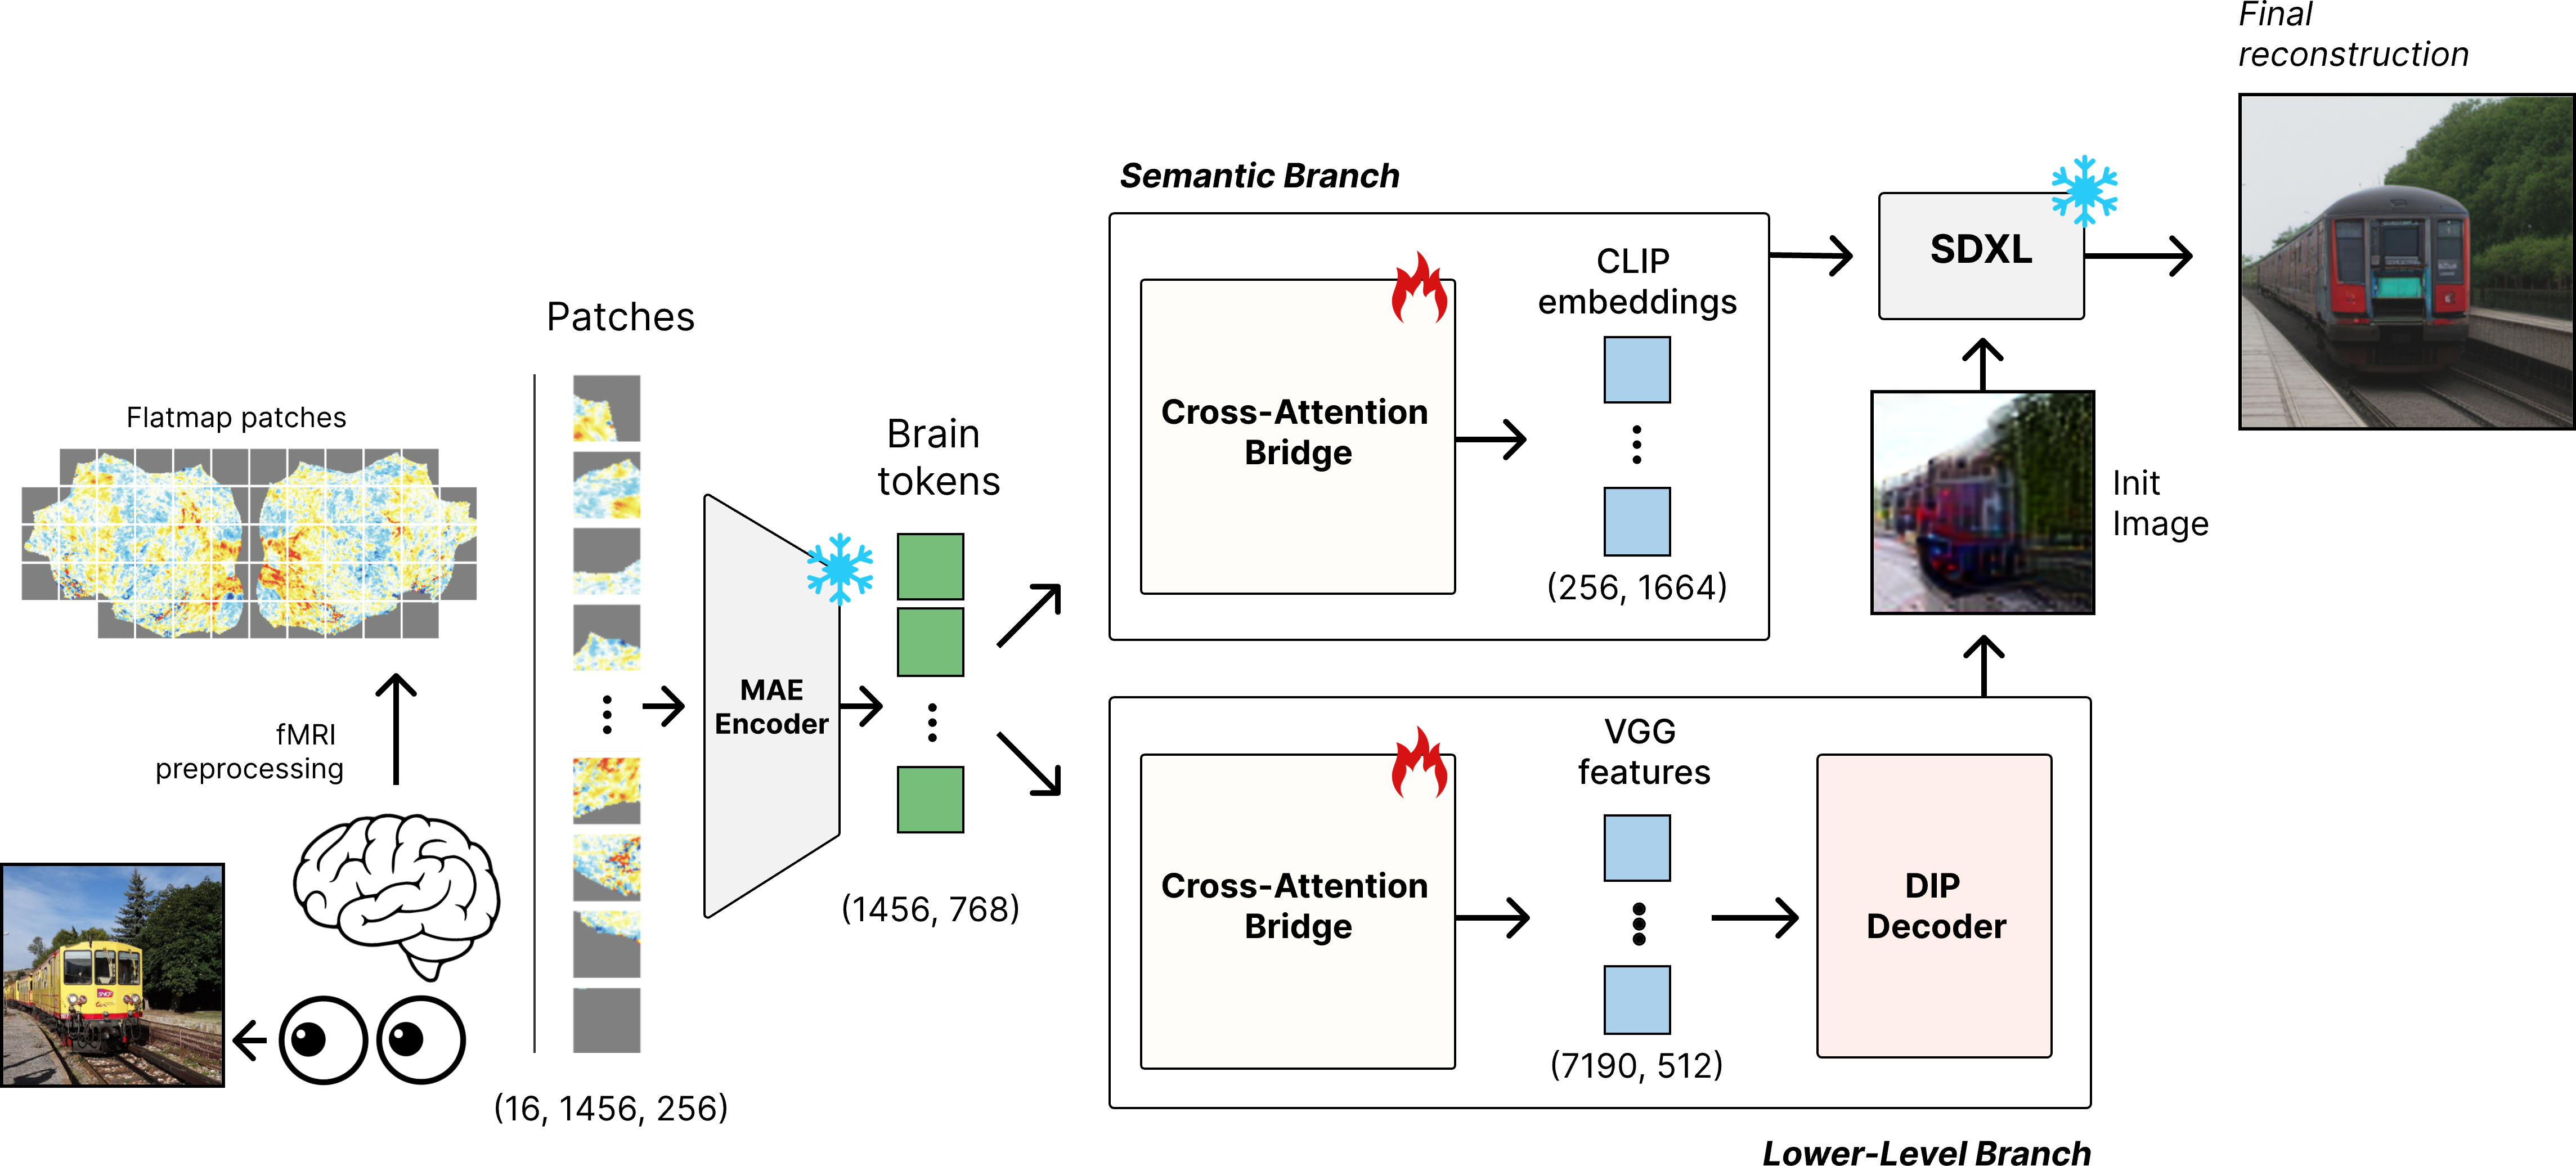
\includegraphics[width=0.75\textwidth]{images/model4.png}
\caption{CortexDecoder overview. A frozen CortexMAE encoder turns cortical flatmap patches into 1456 brain tokens. Two cross-attention bridges, the only trained components, predict OpenCLIP tokens (semantic) and VGG16-BN features (low-level). A DIP-inverted low-level image initializes SDXL-unCLIP, which is conditioned on the predicted OpenCLIP tokens to produce the final image. Images from COCO \cite{lin2015microsoftcococommonobjects} (CC BY 4.0).}
\label{fig:model_schematic}
\end{figure*}

\section{CortexDecoder}
\label{sec:cortex_decoder}
CortexDecoder is a two-branch brain decoding framework that maps cortical flatmap representations to high-level semantic and low-level visual features for image reconstruction. The model first encodes cortical flatmaps using a pretrained CortexMAE encoder, producing spatially organized brain tokens. These brain tokens are then fed into the cross-attention bridge, which predicts visual image features. The semantic branch predicts unpooled CLIP embeddings, while the low-level branch predicts VGG features. Finally, the predicted visual representations are provided to a frozen diffusion decoder to reconstruct the corresponding image.

All model training and evaluations were performed on a single NVIDIA H100 GPU (80 GB). Both branches were trained separately with AdamW \cite{loshchilov2019decoupledweightdecayregularization} (learning rate 5e-4, weight decay 1e-2) and a batch size of 128 under bfloat16 mixed precision. Both the semantic branch and the low-level branch were trained for 25 epochs. Deep Image Prior inversion at inference uses 2,000 Adam steps per image with 36 images optimized in parallel on the GPU.

\subsection{Natural Scenes Dataset}

The Natural Scenes Dataset (NSD) is a large-scale 7T fMRI dataset in which eight participants viewed natural images drawn from MS-COCO (Microsoft Common Objects in Context) \cite{lin2015microsoftcococommonobjects} across up to 40 scan sessions each. Each session comprises 750 trials; in each trial, one image is presented for 3 seconds, followed by a 1-second blank. Each subject viewed 10,000 unique images, each repeated 3 times, for a total of 30,000 trials per subject. A subset of 1000 images (shared1000) was presented to all subjects and is reserved as a standard test set throughout the literature.
The NSD experiment uses a rapid event-related design in which a new image stimulus is presented every 4 seconds, so successive stimuli occur within the timescale of the hemodynamic response. Because the responses to successive trials overlap, single-trial responses cannot be read directly from the time series. A general linear model (GLM) \cite{10.7554/eLife.77599} performs this deconvolution, and its output is a static spatial map of cortical activity per trial rather than a time series. This is precisely the form that 2D flatmap representations and patch-based tokenization assume. We note that the CortexMAE encoder is spatiotemporal and retains a temporal patch dimension from its pretraining on the BOLD time series. However, because our inputs are static single-trial beta maps, we do not utilize this temporal dimension in CortexDecoder.

\subsection{MAE Encoder and Tokenization}
NSD’s surface betas are distributed on a fsaverage mesh \cite{FISCHL2012774} (163,842 vertices per hemisphere). We resample them to fsLR-32k (32,492 vertices per hemisphere, 64,984 total), the standard HCP (Human Connectome Project) \cite{VanEssen_Smith_Barch_Behrens_Yacoub_Ugurbil_2013} mesh on which CortexMAE was pretrained. A pycortex-based \cite{DBLP:journals/fini/GaoHLG15} flat-surface resampler then projects these vertices onto a single-channel $224\times560$ raster, producing the 2D cortical flatmap. Since the projection is defined by a common template mesh rather than by individual anatomy, a given location in the raster corresponds to approximately the same piece of cortex across subjects.
The flatmap is divided into non-overlapping $16\times16$ spatial patches, forming a $14\times35$ grid of 490 cells. Since the cortical surface occupies only part of the bounding box, 364 cells contain cortex and the remaining cells are background. CortexMAE uses a validity mask to exclude these background patches, so only 364 cortical patches are embedded.
CortexMAE is a spatiotemporal masked autoencoder \cite{he2021maskedautoencodersscalablevision} pretrained on BOLD time series. In other words, its patch embedding operates over both space and time. In our case, the input is a single-trial beta map, which has no temporal component. To use the pretrained model, we represent each beta map as a static 16-frame clip. Since we use the CortexMAE encoder out of the box, we also retain its output shape, a sequence of 1456 tokens each with a dimension of 768.

\begin{figure}[!t]
\centering
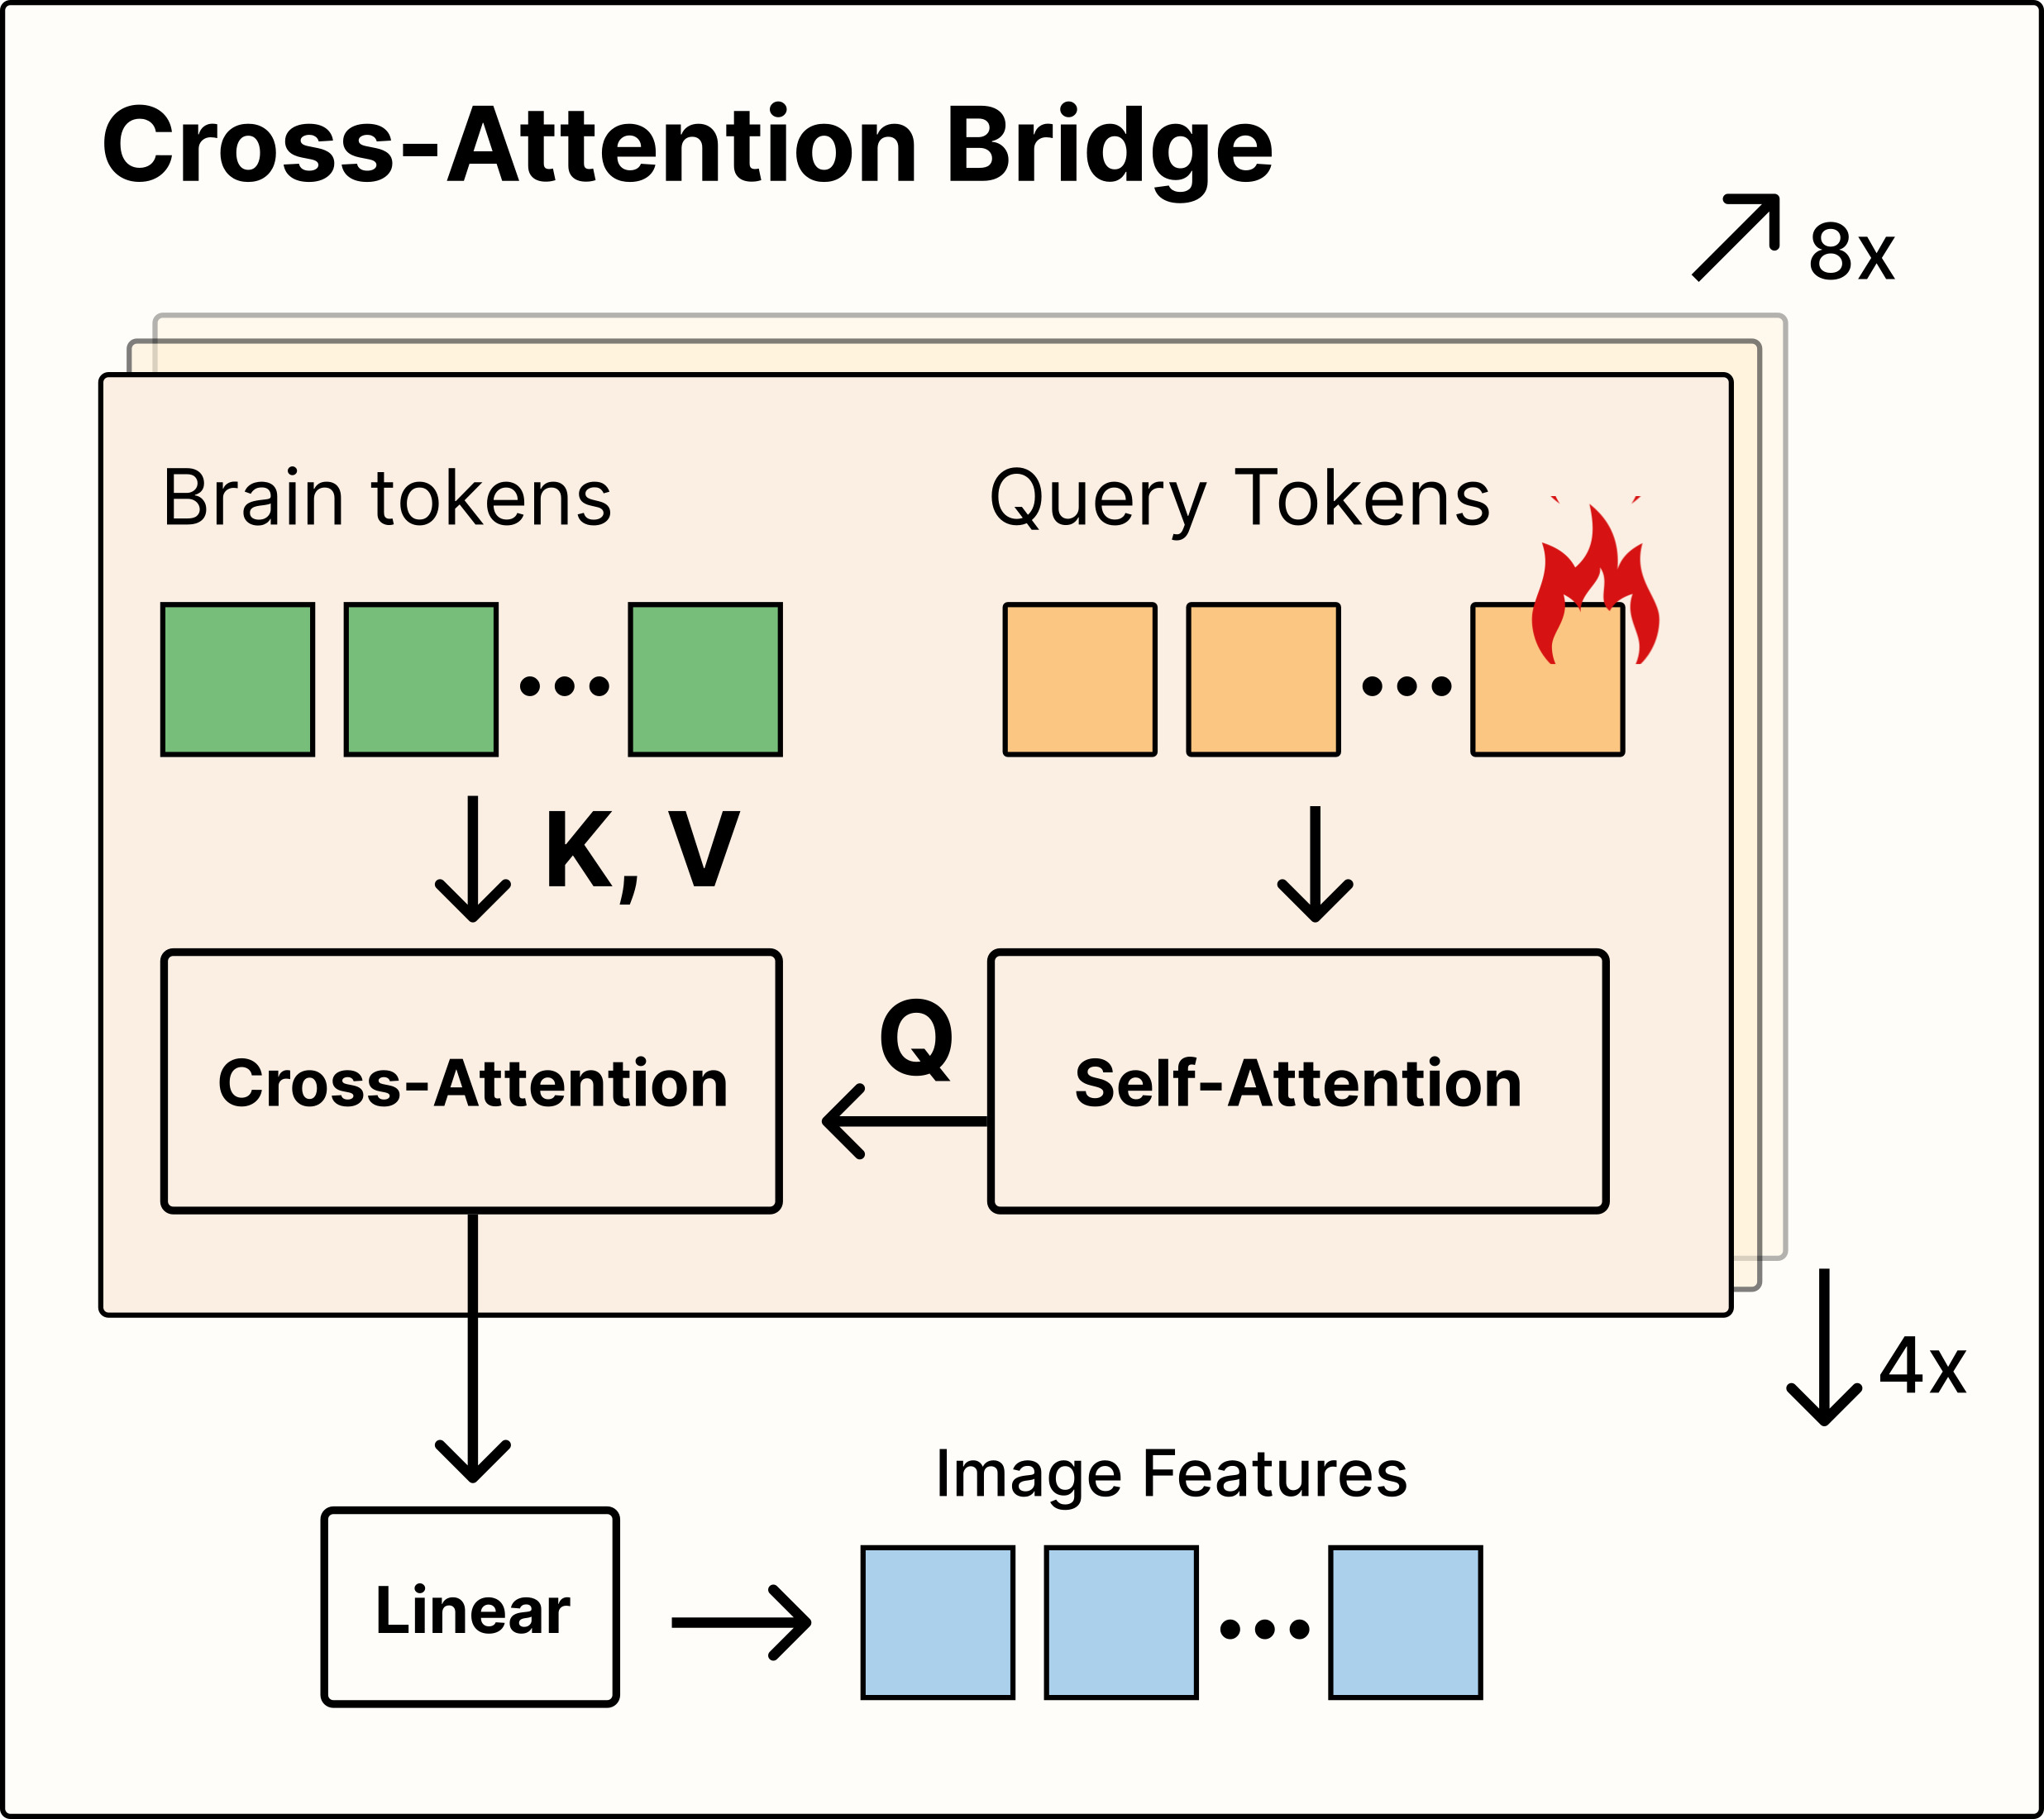
\includegraphics[width=0.8\columnwidth]{images/cross.jpg}
\caption{Cross-attention bridge. Learned queries, one per output token, attend to the brain tokens through 4 blocks of self-attention, cross-attention and FFN. A linear layer projects each query to the target feature dimension. Each branch has its own bridge. Images from COCO \cite{lin2015microsoftcococommonobjects} (CC BY 4.0).}
\label{fig:cross_attention_bridge}
\end{figure}

\subsection{Cross-Attention Bridge}
The bridge maps the sequence of brain tokens to a sequence of visual feature tokens. Its design follows DETR (DEtection TRansformer) \cite{DBLP:journals/corr/abs-2005-12872}. We define a set of learned query vectors with one query per output token. These are randomly initialized and trained jointly with the rest of the model. Each query is responsible for predicting one token of the target visual representation.
The brain tokens serve as memory. They are layer-normalized and projected to the model width when the two dimensions differ. In our case, the CortexMAE embedding dimension and the bridge width are both 768, so no projection is needed. The queries are then passed through a stack of transformer decoder layers. Each layer applies self-attention among the queries, then cross-attention from the queries into the brain memory, and finally a position-wise feed-forward network (FFN). Self-attention lets the queries coordinate with one another so that neighboring output tokens can share information. Cross-attention is where the decoding happens. Each query attends over all 1456 brain tokens and pools the ones that carry information about its target feature. A final linear layer projects each decoded query to the dimensionality of the target representation.
We use 4 decoder layers and 8 attention heads. The model width is 768, with a feed-forward dimension of 3072 and dropout of 0.1. The semantic and low-level branches share these settings.
The key property of this design is that the brain representation remains a sequence throughout the pipeline. Each query attends over the full set of brain tokens. A pooled brain vector would make every query attend to the same input and reduce the decoder to a multilayer perceptron (MLP) applied identically at each output position.

We instantiate the bridge twice with one instance per branch and train the two independently rather than sharing a trunk. The semantic branch uses 256 queries and projects to 1664 dimensions. This matches the shape of the unpooled OpenCLIP ViT-bigG/14 \cite{radford2021learningtransferablevisualmodels, ilharco_gabriel_2021_5143773, schuhmann2022laionb} patch tokens that the diffusion decoder expects as conditioning. The low-level branch uses 7190 queries and projects to 512 dimensions. This matches the concatenated token count of the five VGG16-BN feature layers described in \cref{sec:low_level}. The two branches therefore differ by more than an order of magnitude in output length. They also optimize different losses, since the semantic target is dense and continuous, while the low-level target is better matched by a contrastive objective.

\begin{equation}
\mathcal{L}_{\mathrm{CLIP}} = \mathrm{MSE}\big(\hat{\mathbf{C}}, \mathbf{C}\big),
\end{equation}

\medskip

where $\hat{\mathbf{C}}, \mathbf{C} \in \mathbb{R}^{256 \times 1664}$ are the predicted and target OpenCLIP token sequences, and the error is averaged over all tokens, dimensions and images in the batch.

To train the low-level branch, we extract target tokens from five intermediate layers of a frozen VGG16-BN network (\texttt{relu1\_2} through \texttt{relu5\_3}, totaling $7{,}190$ spatial tokens of dimension $D=512$). For memory efficiency during training, we randomly sub-sample $K\in \{512, 512, 128, 64, 16\}$ query positions per layer at each step and compute a symmetric position-wise InfoNCE contrastive loss across the mini-batch of $B$ trials:

\begin{equation}
\mathcal{L}_{\mathrm{VGG}} =
\frac{1}{2K}\sum_{k=1}^{K}\left[\mathrm{CE}\!\left({\scriptstyle
\frac{\hat{\mathbf{z}}_{:,k}\mathbf{z}_{:,k}^{\top}}{\tau}},
\mathbf{y}\right) + \mathrm{CE}\!\left({\scriptstyle \frac{\mathbf{z}_{:,
k}\hat{\mathbf{z}}_{:,k}^{\top}}{\tau}}, \mathbf{y}\right)\right],
\end{equation}
where $\hat{\mathbf{z}}_{:,k}, \mathbf{z}_{:,k} \in \mathbb{R}^{B \times
D}$ denote the $\ell_2$-normalized predicted and ground-truth feature
matrices at spatial token $k$, $\tau = 0.07$ is the temperature
hyperparameter, and $\mathbf{y} = (1, \dots, B)^{\top}$ indexes the
matching trial pairs across the batch. The final low-level objective
averages $\mathcal{L}_{\mathrm{VGG}}$ equally across all five VGG16-BN layers.

\subsection{Semantic Branch}
The semantic branch predicts the image representations that condition the diffusion decoder. Its target is the unpooled patch-token sequence produced by the OpenCLIP ViT-bigG/14 vision encoder pretrained on LAION-2B \cite{schuhmann2022laionb}. For each stimulus image, we take the 256 patch tokens before the final projection and discard the class (CLS) token. Each token is 1664-dimensional. The bridge therefore uses 256 queries and projects to 1664 dimensions so that its output matches the target.

We use an unpooled token sequence rather than a single pooled embedding. A pooled CLIP vector summarizes an image but discards its spatial layout. A token sequence retains that layout and gives the diffusion decoder a spatially structured conditioning signal. The diffusion decoder we use is a pretrained SDXL-unCLIP model whose cross-attention was trained to condition on exactly 256 bigG tokens of 1664 dimensions. Matching this shape means the decoder can be used frozen with no fine-tuning on our part. Predicting a smaller CLIP variant would require retraining the decoder’s conditioning pathway.

The OpenCLIP encoder is frozen and used only to produce targets. We extract the token sequence for every stimulus image once and cache it. During training, the branch never runs the image encoder. The branch is trained with mean squared error between the predicted and target token sequences, averaged over all 256 positions and 1664 dimensions.

\begin{figure}[h]
\centering
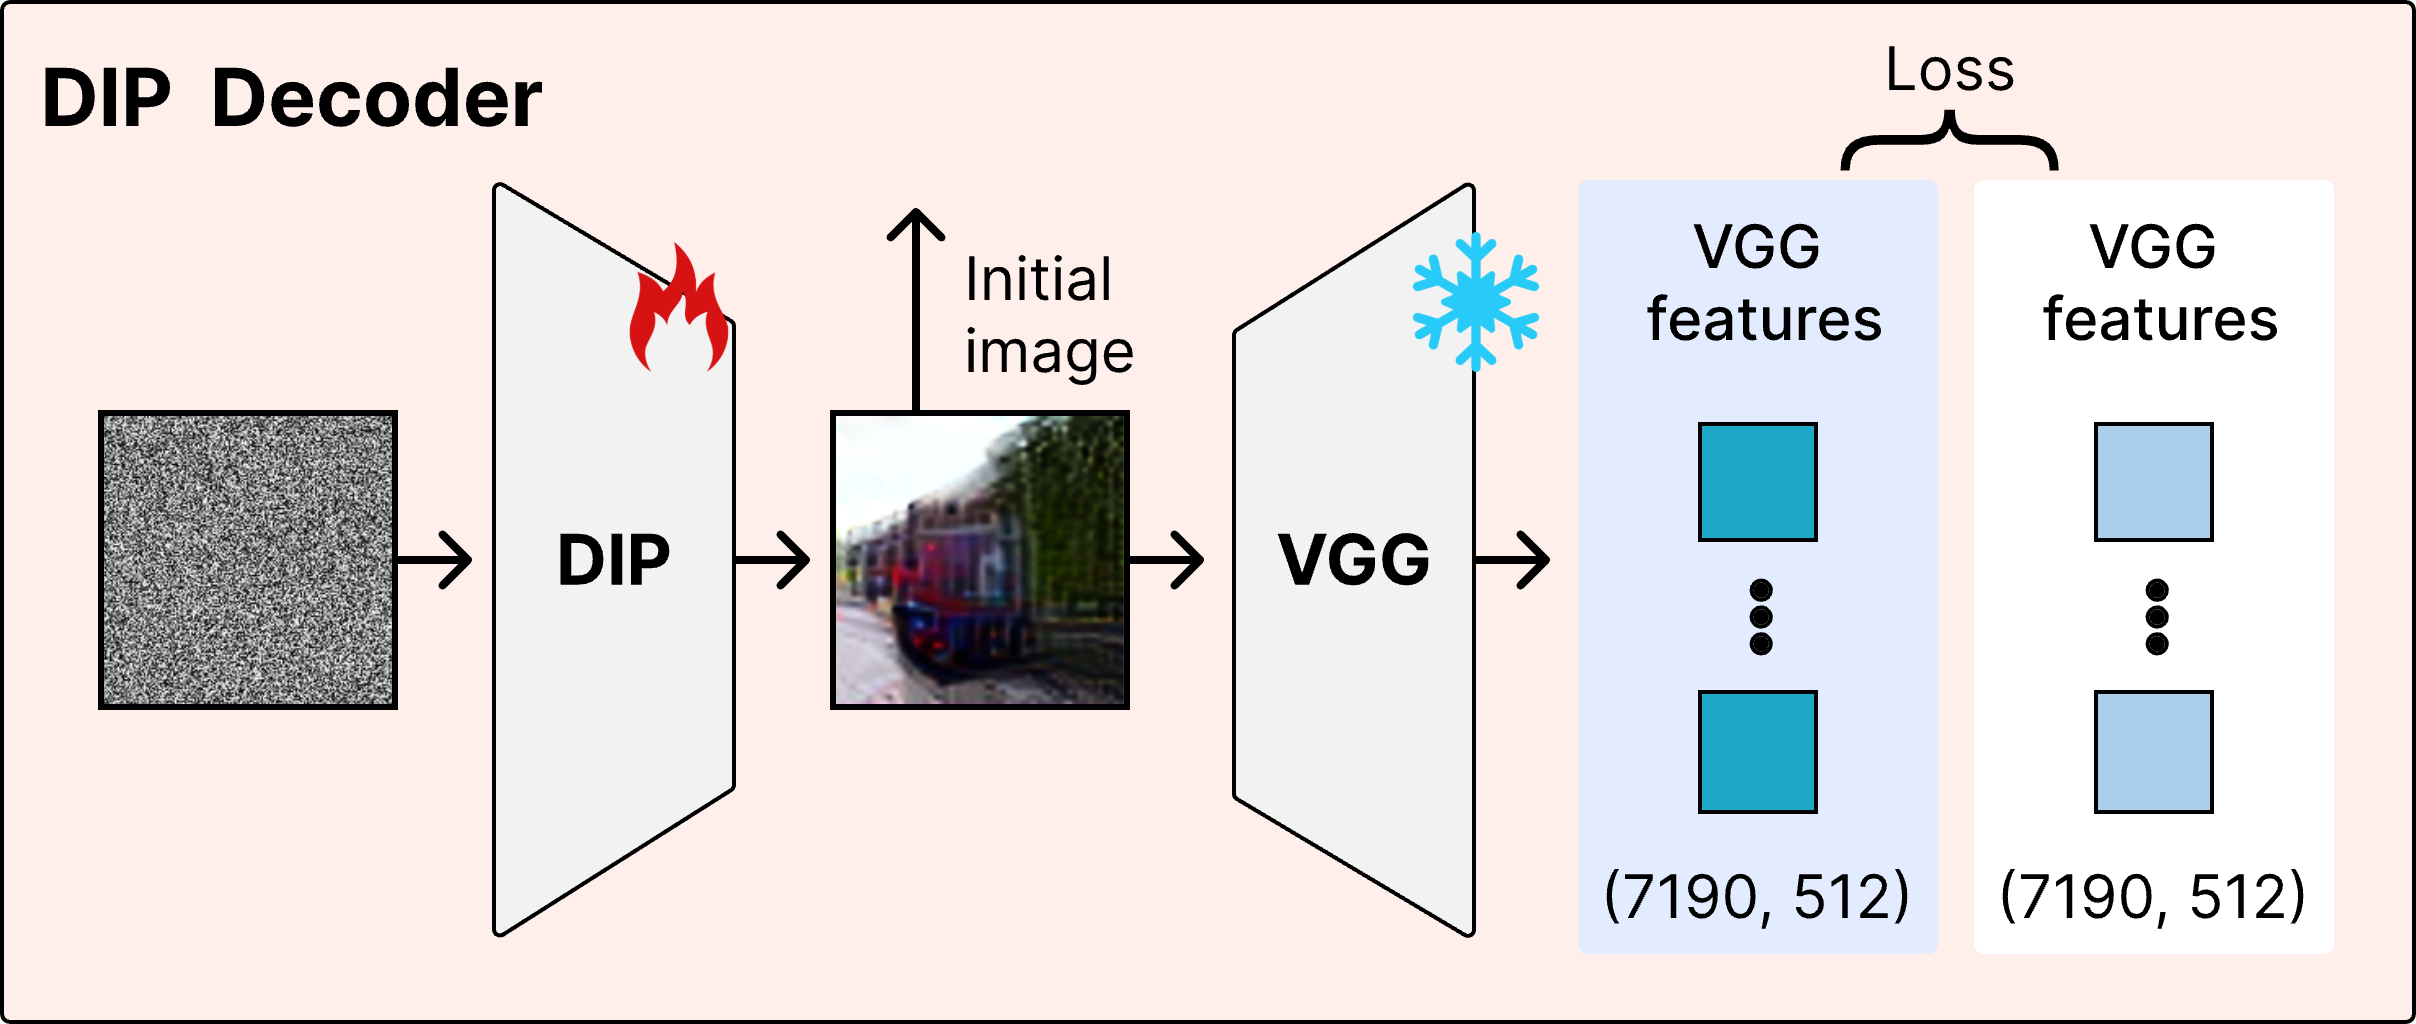
\includegraphics[width=1\columnwidth]{images/DIP3.png}
\caption{Low-level reconstruction with Deep Image Prior. A U-Net maps noise to an image whose frozen VGG16-BN features are matched to the bridge's predicted features. After 2000 optimization steps, its output is the low-level reconstruction.}
\label{fig:dip_reconstruction}
\end{figure}

\subsection{Low-Level Branch}
\label{sec:low_level}
From the predicted VGG feature representation, we reconstruct a low-level image through Deep Image Prior (DIP) inversion. The VGG representation consists of the stacked outputs of five convolutional layers of the VGG16-BN image model.

To convert this representation into the initial image, we optimize a separate DIP U-Net for each image. The U-Net is a small encoder-decoder convolutional generator that maps random Gaussian noise to an RGB image, which is then passed through a frozen VGG16-BN network. The extracted VGG features are compared against the brain-predicted VGG representation using an MSE loss. The gradient is backpropagated only through the DIP U-Net, iteratively updating the generator for a fixed 2000 optimization steps to produce the final low-level reconstruction.

\subsection{Final Image Reconstruction}
To generate the final image reconstruction, we combine the image capturing low-level features generated using DIP with the semantic CLIP prediction using the MindEye2 Stable Diffusion XL unCLIP model (SDXL-unCLIP). SDXL-unCLIP is a pretrained image generation model that generates images from OpenCLIP ViT-bigG/14 image embeddings instead of text-prompt embeddings. The intention is for the low-level DIP image to provide layout, color, and coarse structure while the predicted OpenCLIP ViT-bigG/14 tokens contribute the semantic context of the image.

We first add Gaussian noise to the low-level image to partially corrupt fine detail while preserving coarse layout and color. This re-noised image becomes the initial state for SDXL-unCLIP, anchoring the image structure. The predicted OpenCLIP token representation then steers the denoising process toward the correct semantic context, turning the blurry low-level reconstruction into a detailed final image. With this approach, the reconstruction should reflect both the content and the structure of the stimulus. We run this diffusion process multiple times for each image and select the reconstruction whose downscaled version has the lowest MSE relative to the low-level reconstruction. This keeps the final image from straying too far from the predicted low-level image structure.

\begin{figure}[!t]
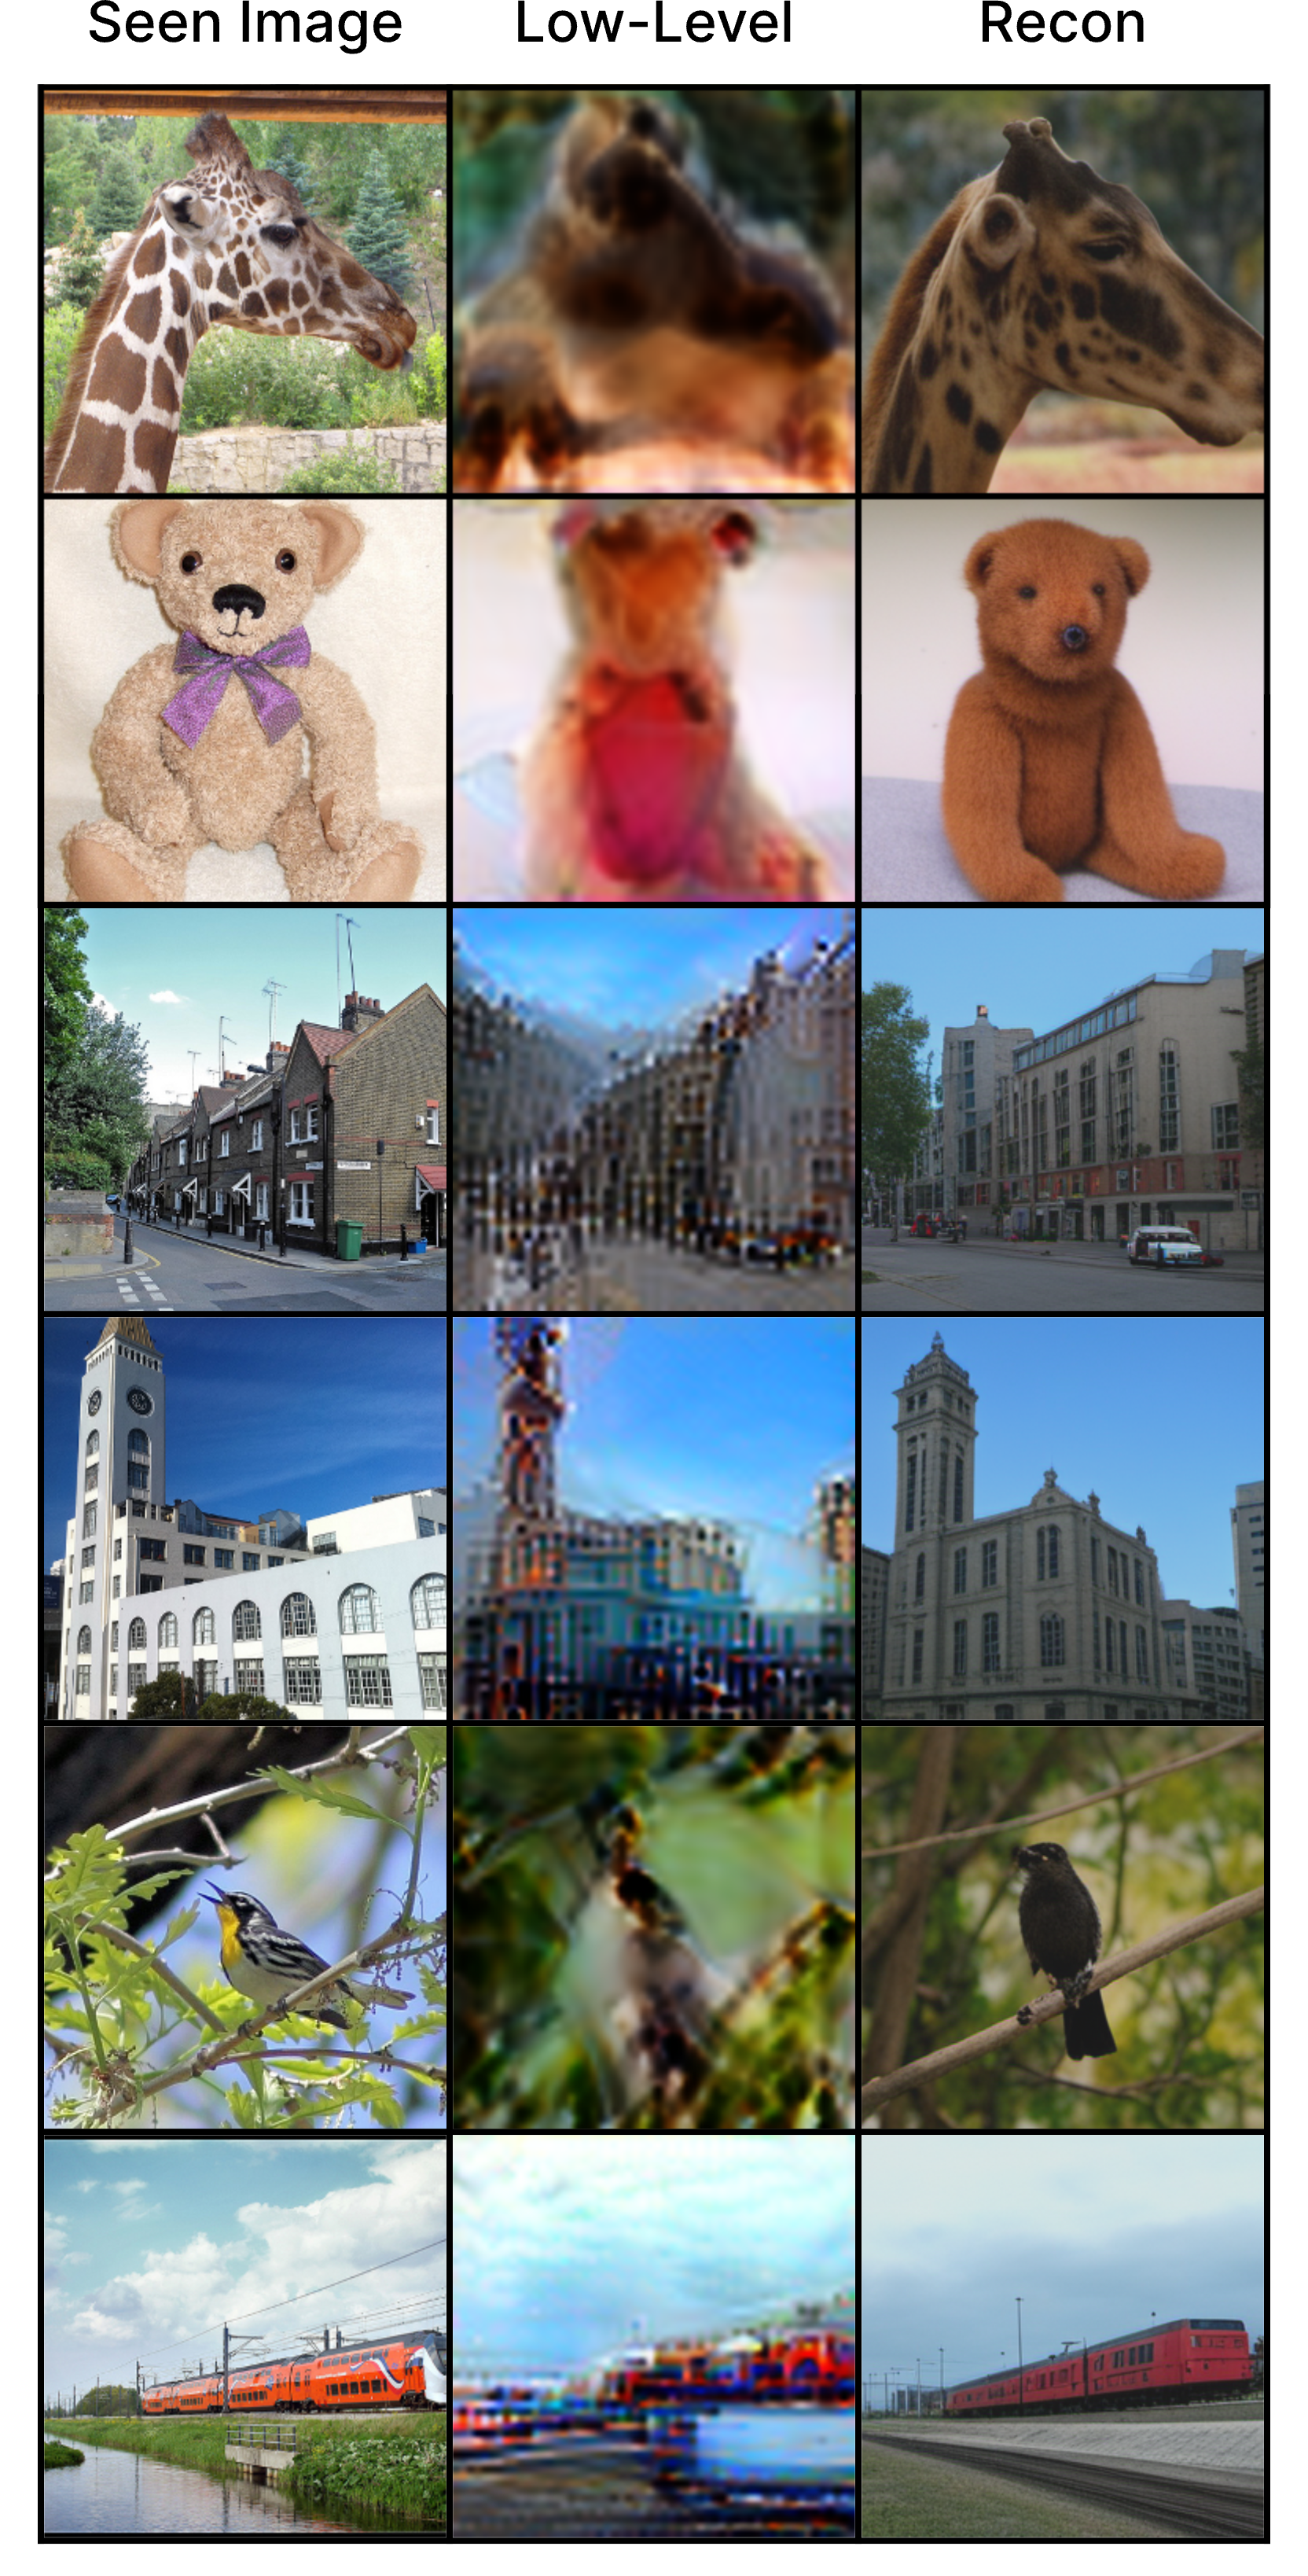
\includegraphics[width=0.65\columnwidth]{images/stacked_triptych_collage3.png}
\centering
\caption{Stimulus (left), low-level DIP reconstruction (middle) and final diffusion reconstruction (right). Images from COCO \cite{lin2015microsoftcococommonobjects} (CC BY 4.0).}
\label{fig:stacked_triptych}
\end{figure}


% You must include your signed IEEE copyright release form when you submit your finished paper.
% We MUST have this form before your paper can be published in the proceedings.

% Please direct any questions to the production editor in charge of these proceedings at the IEEE Computer Society Press:
% \url{https://www.computer.org/about/contact}.

\section{Results}
\label{sec:results}

\begin{table*}[!t]
\centering
\footnotesize
\renewcommand{\arraystretch}{1.25}
\setlength{\tabcolsep}{3pt}
\begin{tabular*}{\textwidth}{@{\extracolsep{\fill}}llcccccccc@{}}
\toprule
& & \multicolumn{4}{c}{Low-Level} & \multicolumn{4}{c}{High-Level} \\
\cmidrule(lr){3-6}\cmidrule(lr){7-10}
\multicolumn{2}{l}{\textbf{Method}}
& PixCorr$\uparrow$ & SSIM$\uparrow$ & Alex(2)$\uparrow$ & Alex(5)$\uparrow$
& Incep$\uparrow$ & CLIP$\uparrow$ & Eff$\downarrow$ & SwAV$\downarrow$ \\
\midrule
\multirow{5}{*}{\shortstack{Voxel-\\based}}
& Takagi \textit{et al.}$^\ddagger$ (CVPR'23) \cite{10205187}
& 0.246 & 0.410 & 78.9\% & 85.6\%
& 83.8\% & 82.1\% & 0.811 & 0.504 \\
& Brain-Diffuser$^\ddagger$ (Sci-Rep'23) \cite{ozcelik2023brain}
& 0.273 & 0.365 & 94.4\% & 96.6\%
& 91.3\% & 90.9\% & 0.728 & 0.421 \\
& MindEye$^\ddagger$ (NeurIPS'23) \cite{scotti2023reconstructingmindseyefmritoimage}
& 0.319 & 0.360 & 92.8\% & 96.9\%
& 94.6\% & \underline{93.3\%} & 0.648 & 0.377 \\
& MindEye2$^\dagger$ (ICML'24) \cite{scotti2024mindeye2sharedsubjectmodelsenable}
& \underline{0.322} & \underline{0.431} & 96.1\% & \underline{98.6\%}
& \underline{95.4\%} & 93.0\% & \underline{0.619} & \underline{0.344} \\
& Brain-IT$^\dagger$ (arXiv'25) \cite{beliy2025brainitimagereconstructionfmri}
& \textbf{0.386} & \textbf{0.486} & \textbf{98.4\%} & \textbf{99.5\%}
& \textbf{97.3\%} & \textbf{96.4\%} & \textbf{0.564} & \textbf{0.320} \\
\midrule
\multirow{3}{*}{Flat-map}
& NeuroPictor$^\dagger$ (ECCV'24) \cite{huo2024neuropictorrefiningfmritoimagereconstruction}
& 0.229 & 0.375 & \underline{96.5\%} & 98.4\%
& 94.5\% & \underline{93.3\%} & 0.639 & 0.350 \\
& \textbf{CortexDecoder (Low-Level)}
& 0.321 & 0.393 & 94.4\% & 97.9\%
& 89.7\% & 74.3\% & 0.856 & 0.590 \\
& \textbf{CortexDecoder (Final)}
& 0.311 & 0.408 & 93.2\% & 96.1\%
& 91.4\% & 89.9\% & 0.697 & 0.404 \\
\bottomrule
\end{tabular*}
\caption{Reconstruction metrics on NSD shared1000. CortexDecoder results are averaged over Subjects 1 and 2; baseline results are averaged over Subjects 1, 2, 5 and 7. Baselines are grouped by fMRI input representation and taken as reported by each paper, except $^\ddagger$, which are recomputed by MindEye2 \cite{scotti2024mindeye2sharedsubjectmodelsenable} on the full 40 sessions. \textbf{Bold}: best; \underline{underline}: second best. $^\dagger$Pretrains on multiple subjects.}
\label{tab:reconstruction}
\end{table*}


We evaluate CortexDecoder on the NSD shared1000 test set, which is kept completely separate from the training and validation data to prevent leakage. All metrics compare reconstructions against the stimulus images viewed by each subject, and we report the average over Subjects 1 and 2. We report PixCorr (Pixel Correlation), SSIM (Structural Similarity Index Measure) \cite{1284395}, AlexNet(2), AlexNet(5) \cite{NIPS2012_c399862d}, InceptionV3 \cite{szegedy2015rethinkinginceptionarchitecturecomputer}, CLIP \cite{radford2021learningtransferablevisualmodels}, EfficientNet-B1 \cite{tan2020efficientnetrethinkingmodelscaling} and SwAV-ResNet50 \cite{caron2021unsupervisedlearningvisualfeatures}. PixCorr and SSIM measure pixel and structural similarity while AlexNet, InceptionV3 and CLIP measure feature-space similarity. EfficientNet and SwAV report correlation distance, where lower is better.

We report metrics for both the low-level DIP reconstruction and the final diffusion reconstruction. This allows us to evaluate the contribution of the low-level branch separately from the semantic conditioning. Because diffusion is stochastic, we generate ten candidates per image. Then we select the generated image with the lowest pixelwise MSE to the low-level reconstruction after resizing. This approach does not use ground-truth images and favors candidates that preserve the predicted structure.

\subsection{Reconstruction Benchmarks}
CortexDecoder is competitive with prior methods in capturing low-level and mid-level features in reconstructed images. Specifically, our model performs well on PixCorr and SSIM, reflecting the contribution of the low-level branch. However, it is weaker at capturing semantic features in the reconstructed images.

The results show that introducing semantic conditioning degrades low-level fidelity. For example, the low-level reconstruction on its own scores higher on most low-level metrics (PixCorr, AlexNet(2) and AlexNet(5)) than the final reconstruction, where semantic conditioning is introduced in the diffusion stage. We conclude that the final reconstruction, which combines semantic and low-level representations, improves on semantic metrics at the expense of low-level performance.



\section{Conclusion}
\label{sec:conclusion}
We introduce CortexDecoder, an fMRI-to-image reconstruction framework that uses 2D cortical flatmaps as neural representations for visual decoding. By converting cortical flatmaps into patch tokens, CortexDecoder enables the use of Vision Transformers while preserving the spatial structure of cortical responses. A pretrained CortexMAE encoder produces brain tokens, which are then mapped through two cross-attention branches: one for semantic features and one for low-level image reconstruction. These predictions are then passed to a fine-tuned SDXL-unCLIP image generation model, which takes the predicted low-level image as its initial image and generates the final reconstruction conditioned on the predicted semantic embedding.

Our results show that cortical flatmaps preserve enough information to support brain decoding. CortexDecoder is strongest at low-level reconstruction, particularly on the PixCorr and SSIM metrics, across the two subjects we evaluated. Overall, flatmaps are a promising fMRI representation for brain decoding, as we have demonstrated for image reconstruction.

\section{Limitations}
\label{sec:limitations}

Due to compute and budget constraints, our experiments are limited to NSD Subjects 1 and 2, instead of the full four-subject evaluation used in the prior works discussed above. Our results in \cref{tab:reconstruction} are therefore averaged over two subjects, while the baselines are averaged over four, so the comparison is not strictly like-for-like. A clear direction for future work is to extend our method to all four subjects and evaluate whether the observed patterns hold across them.

Additionally, our compute and budget constraints restricted hyperparameter tuning, design iteration, and the repeated full evaluations that would have helped optimize our metrics. We were only able to perform one full evaluation run, rather than multiple design iterations, which may partially explain the gap to other state-of-the-art models on the high-level metrics.
\section{Future Work}
\label{sec:future_work}

In future work, we will extend our experiments from NSD Subjects 1 and 2 to the full four-subject setting used by other papers. This would evaluate whether the observed performance of our pipeline holds up across subjects with differing brain anatomies.

We would likely implement this by introducing a functional clustering space shared across subjects. Specifically, we would summarize each flatmap patch across trials into a single descriptor vector, then fit a Gaussian Mixture Model \cite{dempster1977maximum} to map brain patches from all subjects into a common cluster space. A cross-attention layer could then compress the patches assigned to each cluster into a fixed set of cluster tokens. Similar strategies have proven effective in prior work for training a single transferable model across many subjects \cite{beliy2026wisdomcrowdbrainsuniversal, beliy2025brainitimagereconstructionfmri}.

Together, these extensions would enable a more direct comparison against prior multi-subject methods and test whether our approach remains competitive at scale.

Another direction is to replace CLIP as the target semantic representation with the embedding space of a more recent model such as SigLIP2 \cite{tschannen2025siglip2multilingualvisionlanguage}. One limitation of our current pipeline is that semantic conditioning on CLIP embeddings comes at the expense of low-level performance. Replacing CLIP with a stronger semantic embedding model such as SigLIP2 could improve visual-semantic alignment and, in turn, performance on both low-level and high-level evaluations. This may require training an SDXL decoder that accepts SigLIP2 embeddings as conditioning inputs.

\begin{figure}[!t]
\centering
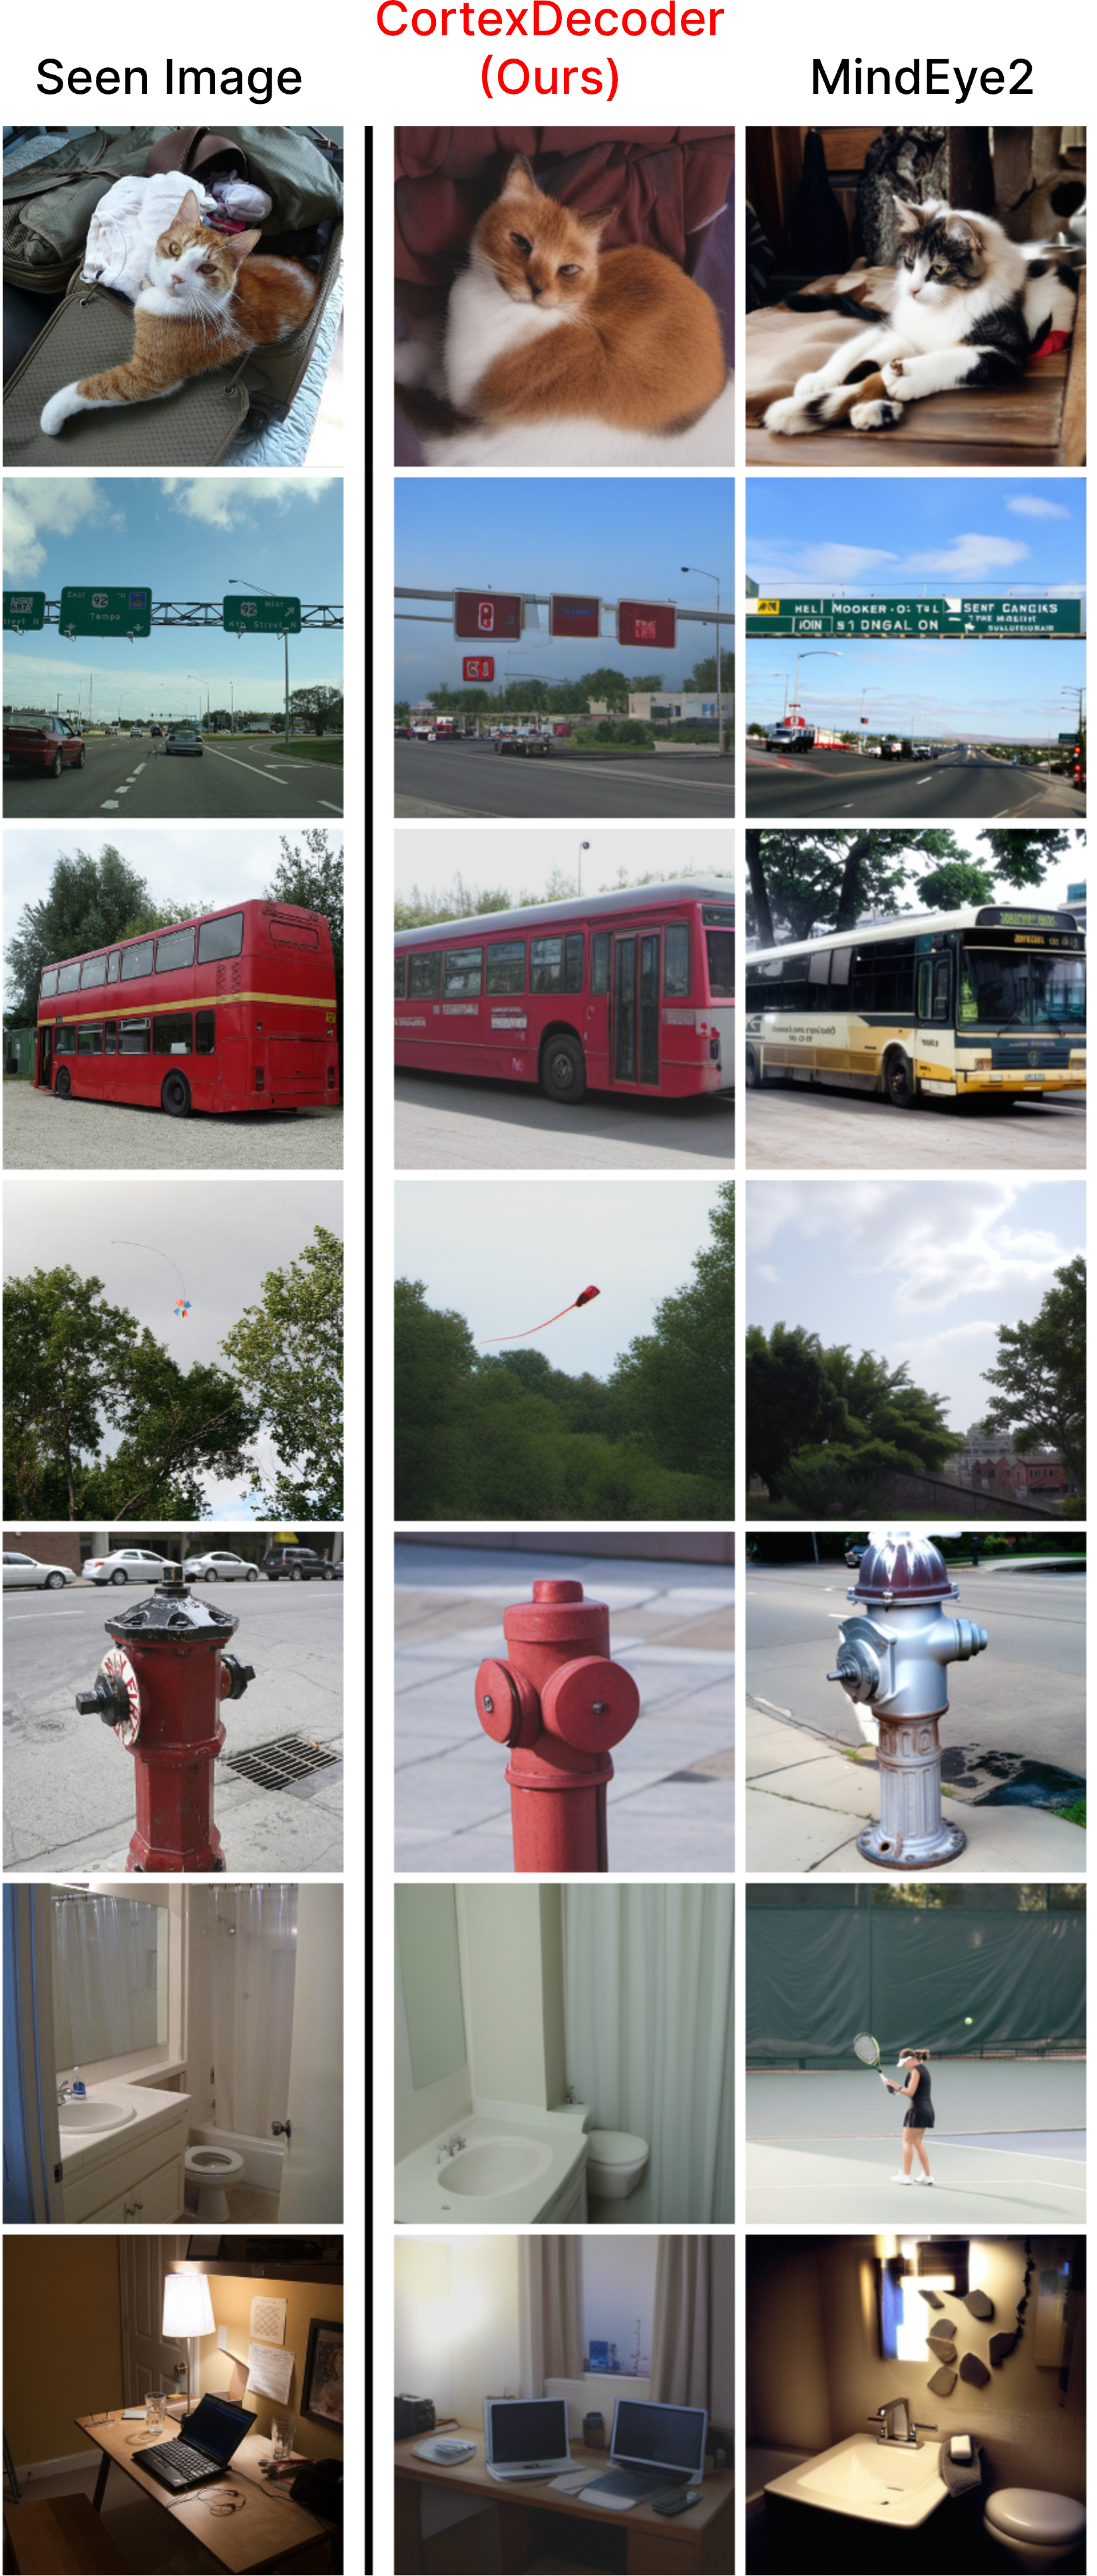
\includegraphics[width=0.8\columnwidth]{images/comparison4.png}
\caption{Stimulus (left), CortexDecoder (middle) and MindEye2 (right) reconstructions. Images from COCO \cite{lin2015microsoftcococommonobjects} (CC BY 4.0).}
\label{fig:comparison}
\end{figure}

{
    \small
    \bibliographystyle{ieeenat_fullname}
    \bibliography{main}
}


\end{document}
